\section{实验结果与分析}
\subsection{Cache仿真结果分析}
\subparagraph{仿真代码设计}
为了实现Cache正确性的仿真验证,本次实验采用了对Cache和CMU模块的单独仿真。仿真代码的设计如下:
\begin{lstlisting}[language=Verilog]
    module cmu_sim (
        input wire clk,
        input wire rst,
        output reg [7:0] clk_count = 0,
        output reg [7:0] inst_count = 0,
        output reg [7:0] hit_count = 0
        );
        
        // instruction
        reg [3:0] index = 0;
        wire valid;
        wire write;
        wire [31:0] addr;
        wire [2:0] u_b_h_w;
        wire stall;
        inst INST (
            .clk(clk),
            .rst(rst),
            .index(index),
            .valid(valid),
            .write(write),
            .addr(addr),
            .u_b_h_w(u_b_h_w)
        );
    
        always @(posedge clk) begin
            if (rst)
                index <= 0;
            else if (valid && ~stall)
                index <= index + 1'h1;
        end
        // ram
        wire mem_cs;
        wire mem_we;
        wire [31:0] mem_addr;
        wire [31:0] mem_din;
        wire [31:0] mem_dout;
        wire mem_ack;
        data_ram RAM (
            .clk(clk),
            .rst(rst),
            .addr({21'b0, mem_addr[10:0]}),
            .cs(mem_cs),
            .we(mem_we),
            .din(mem_din),
            .dout(mem_dout),
            .stall(),
            .ack(mem_ack),
            .ram_state()
        );
        
        // cache
        wire [31:0] data_r;
        cmu CMU (
            .clk(clk),
            .rst(rst),
            .addr_rw(addr),
            .u_b_h_w(u_b_h_w),
            .en_r(~write),
            .data_r(data_r),
            .en_w(write),
            .data_w({16'h5678, clk_count, inst_count}),
            .stall(stall),
            .mem_cs_o(mem_cs),
            .mem_we_o(mem_we),
            .mem_addr_o(mem_addr),
            .mem_data_i(mem_dout),
            .mem_data_o(mem_din),
            .mem_ack_i(mem_ack),
            .cmu_state()
        );
    
        // counter
        reg stall_prev;
        
        always @(posedge clk) begin
            if (rst)
                stall_prev <= 0;
            else
                stall_prev <= stall;
        end
        
        always @(posedge clk) begin
            if (rst) begin
                clk_count <= 0;   // 时钟计数
                inst_count <= 0;  // 指令计数
                hit_count <= 0;   // 命中计数
            end
            else if (valid) begin
                clk_count <= clk_count + 1'h1;
                inst_count <= index + 1'h1;
                if (~stall_prev && ~stall)
                    hit_count <= hit_count + 1'h1;
            end
        end
    
    endmodule    
\end{lstlisting}

为了验证结果,本次实验还设计了一个单独的Test Bench以供测试:
\begin{lstlisting}[language=verilog]
module inst (
    input wire clk,
    input wire rst,
    input wire [3:0] index,  // instruction index
    output wire valid,  // stop running if valid is 0
    output wire write,  // write enable signal for cache
    output wire [31:0] addr,  // address for cache
    output wire [2:0] u_b_h_w
    );
    reg [39:0] data [0:9];
    initial begin
        data[0] = 40'h0_2_00000004;  // read miss               1+17
        data[1] = 40'h0_3_00000019;  // write miss              1+17
        data[2] = 40'h1_2_00000008;  // read hit                1
        data[3] = 40'h1_3_00000014;  // write hit               1
        
        data[4] = 40'h2_2_00000204;  // read miss               1+17
        data[5] = 40'h2_3_00000218;  // write miss              1+17
        data[6] = 40'h0_3_00000208;  // write hit               1
        data[7] = 40'h4_2_00000414;  // read miss + dirty       1+17+17
        data[8] = 40'h1_3_00000404;  // write miss + clean      1+17
        data[9] = 40'h0;           // end                     total: 128
    end
    assign
        u_b_h_w = data[index][38:36],
        valid = data[index][33],
        write = data[index][32],
        addr = data[index][31:0];
        
endmodule
\end{lstlisting}

\subparagraph{仿真结果分析}
根据上述仿真代码,实验的仿真结果如下,在此部分我组将对仿真结果进行逐一分析。
首先同样是多周期的重置过程,以保证cache与内存内容的彻底重置。
\begin{figure}[H] %H为当前位置,!htb为忽略美学标准,htbp为浮动图形
	\centering %图片居中
	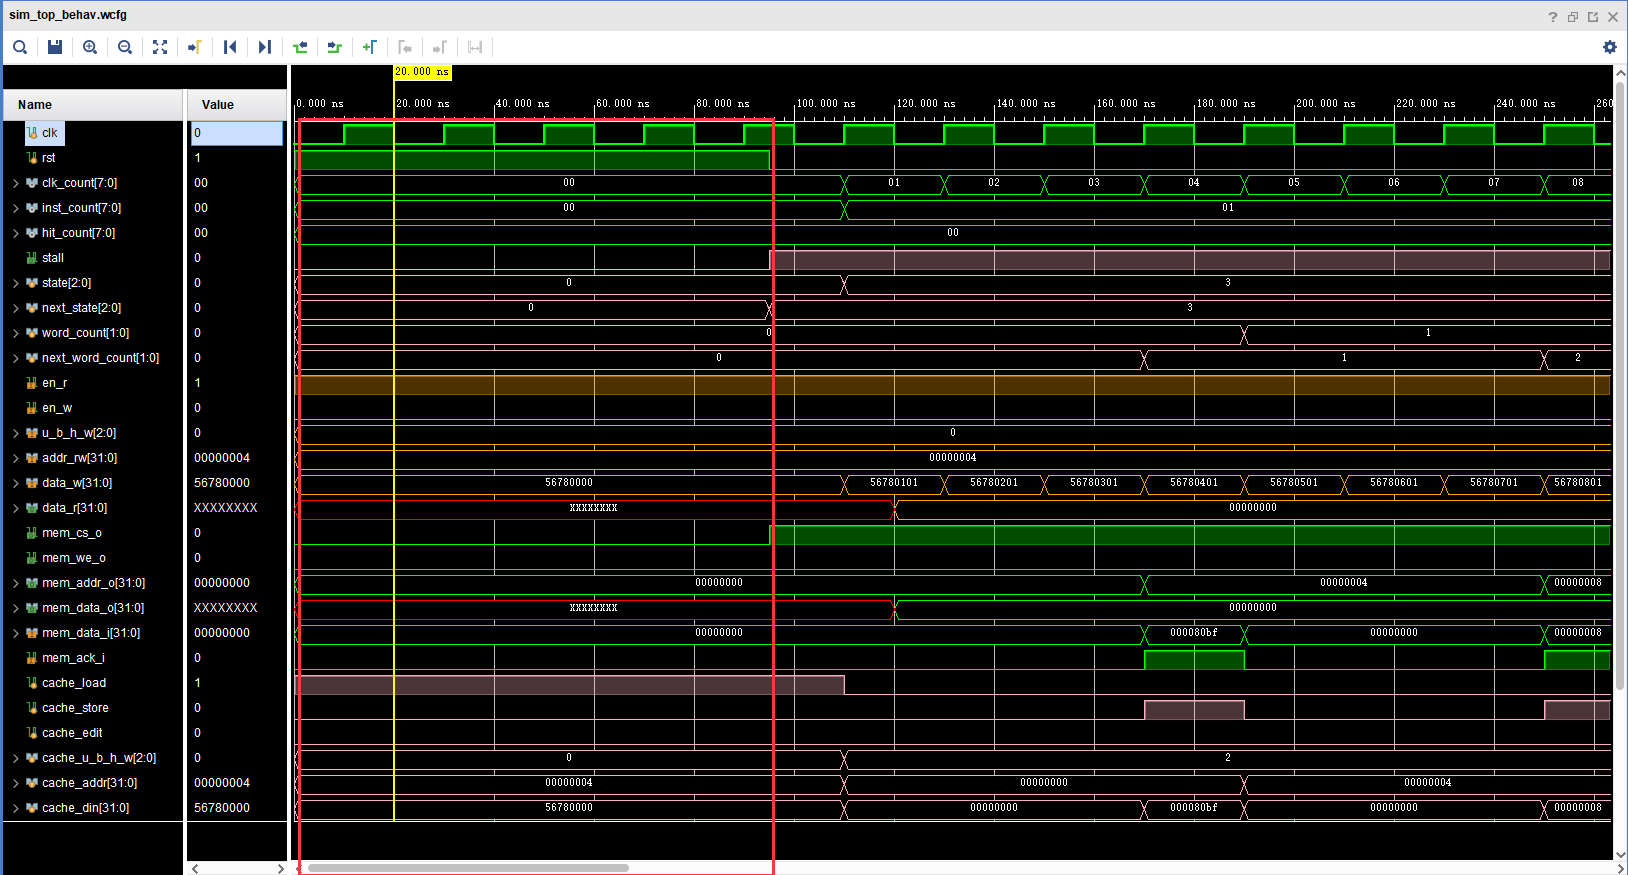
\includegraphics[width=1.0\textwidth]{figs/sres1.png} %插入图片,[]中设置图片大小,{}中是图片文件名
	\caption{重置过程} %最终文档中希望显示的图片标题
	\label{Fig.4} %用于文内引用的标签
\end{figure}

在95ns后,重置过程结束,此时将会进入第一个状态,对应Test Bench中第一条cache访问的执行,此时我们可以看到mem\_cs\_o信号
已经升起,由于第一次内存访问是read操作并且是read miss,所以可以看到next\_state已经被置为了3(S\_FILL),准备从memory中读取
数据,并且此时cmu的stall信号升起,仿真结果正确。

\begin{figure}[H]
    \centering
    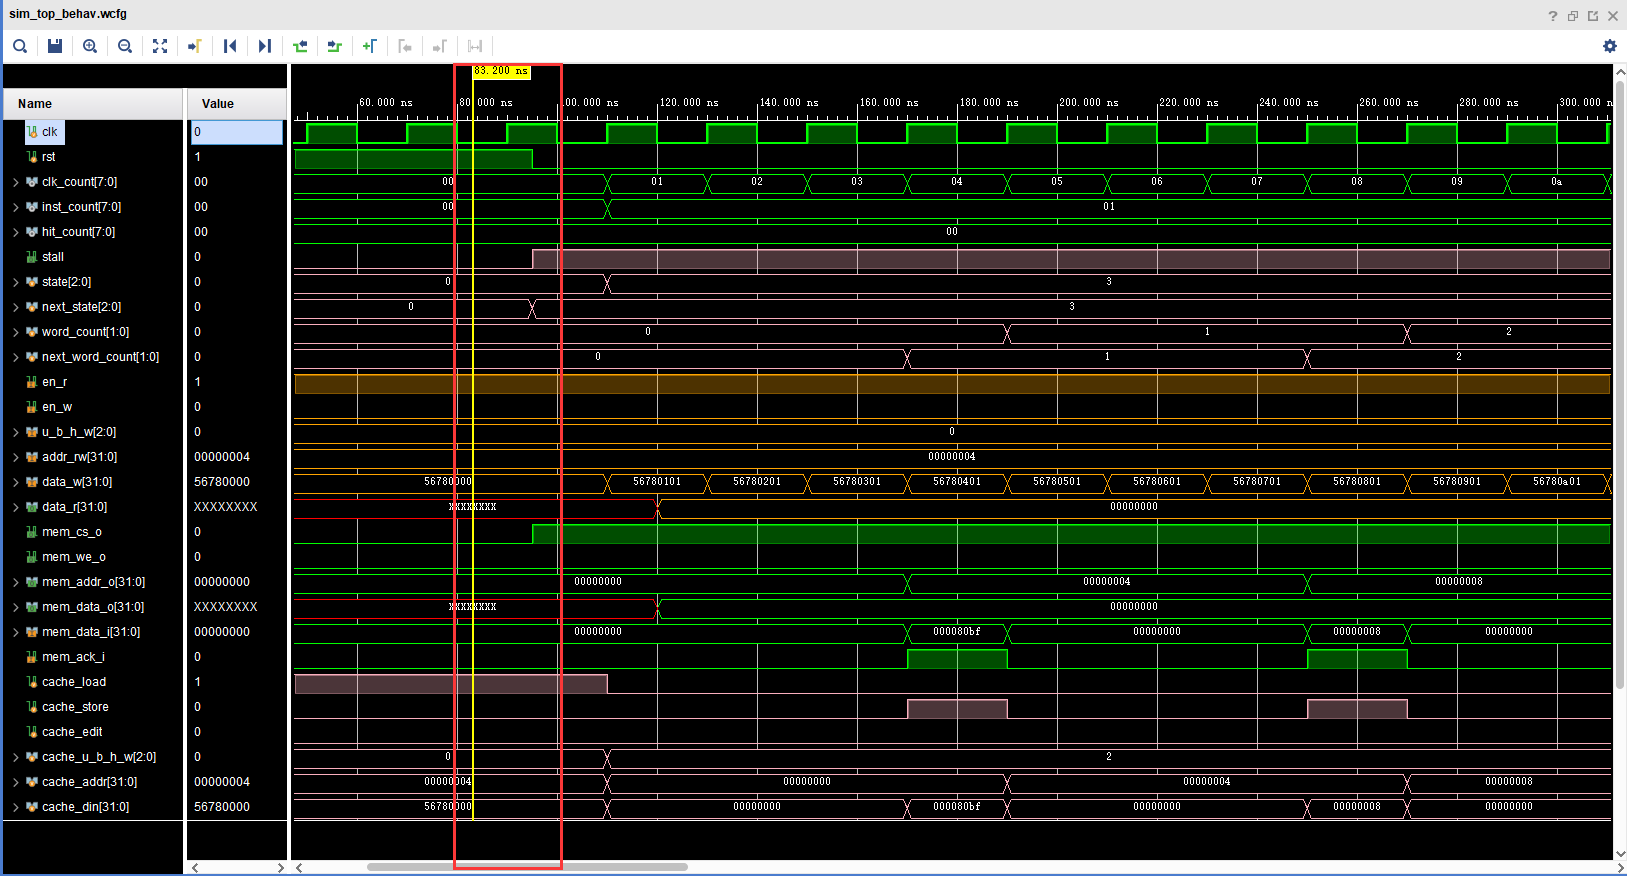
\includegraphics[width=1.0\textwidth]{figs/sres2.png}
    \caption{read miss}
    \label{Fig.5}
\end{figure}

S\_FILL状态在上升沿从memory读取数据,下降沿向cache写入数据,由计数器控制直到整个cache line全部写入。由于每个Word的读取需要
4个时钟周期,而一个Data Line中含有4个Word,所以此过程需要16个时钟周期完成,我们可以从仿真图上看到word\_count的值从0到3,并且在
每次读Word的最后一个周期mem\_ack和cache\_store信号都升起,说明已经从内存中得到一个Word并准备写入cache,仿真结果正确。

\begin{figure}[H]
    \centering
    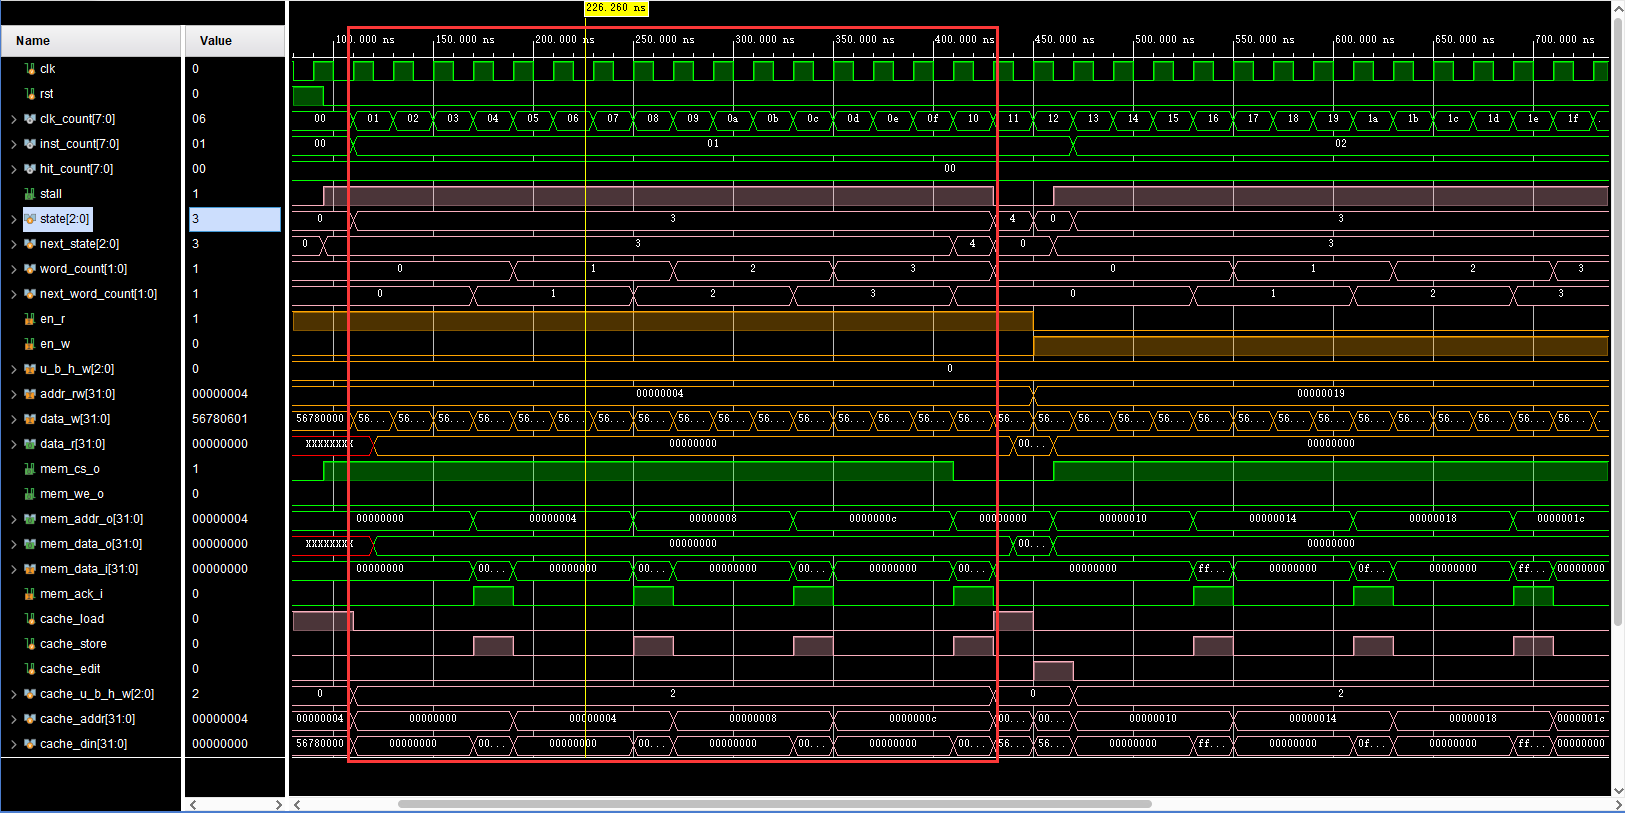
\includegraphics[width=1.0\textwidth]{figs/sres3.png}
    \caption{S\_FILL}
    \label{Fig.6}
\end{figure}

接下来进入S\_WAIT状态,执行之前由于miss而不能进行的cache操作。此时state为4(S\_WAIT),
并且cache\_load信号重新升起,并且stall信号降下仿真结果正确。

\begin{figure}[H]
    \centering
    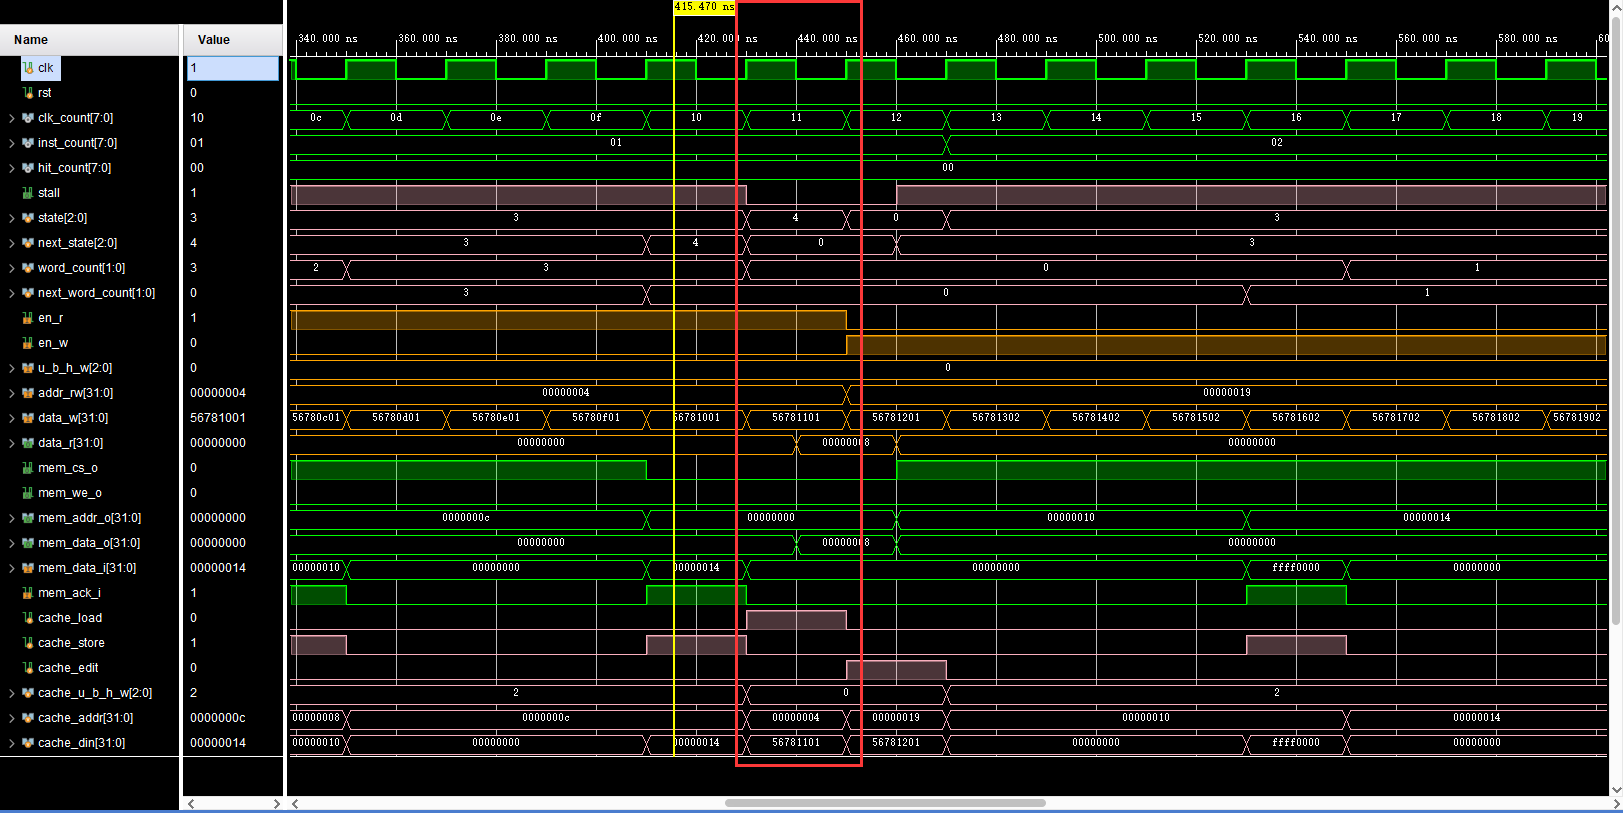
\includegraphics[width=1.0\textwidth]{figs/sres4.png}
    \caption{S\_WAIT}
    \label{Fig.7}
\end{figure}

接下来仿真Write Miss的情形,可以看到此时en\_w和cache\_load信号升起,cache addr也变为0x19

\begin{figure} [H]
    \centering
    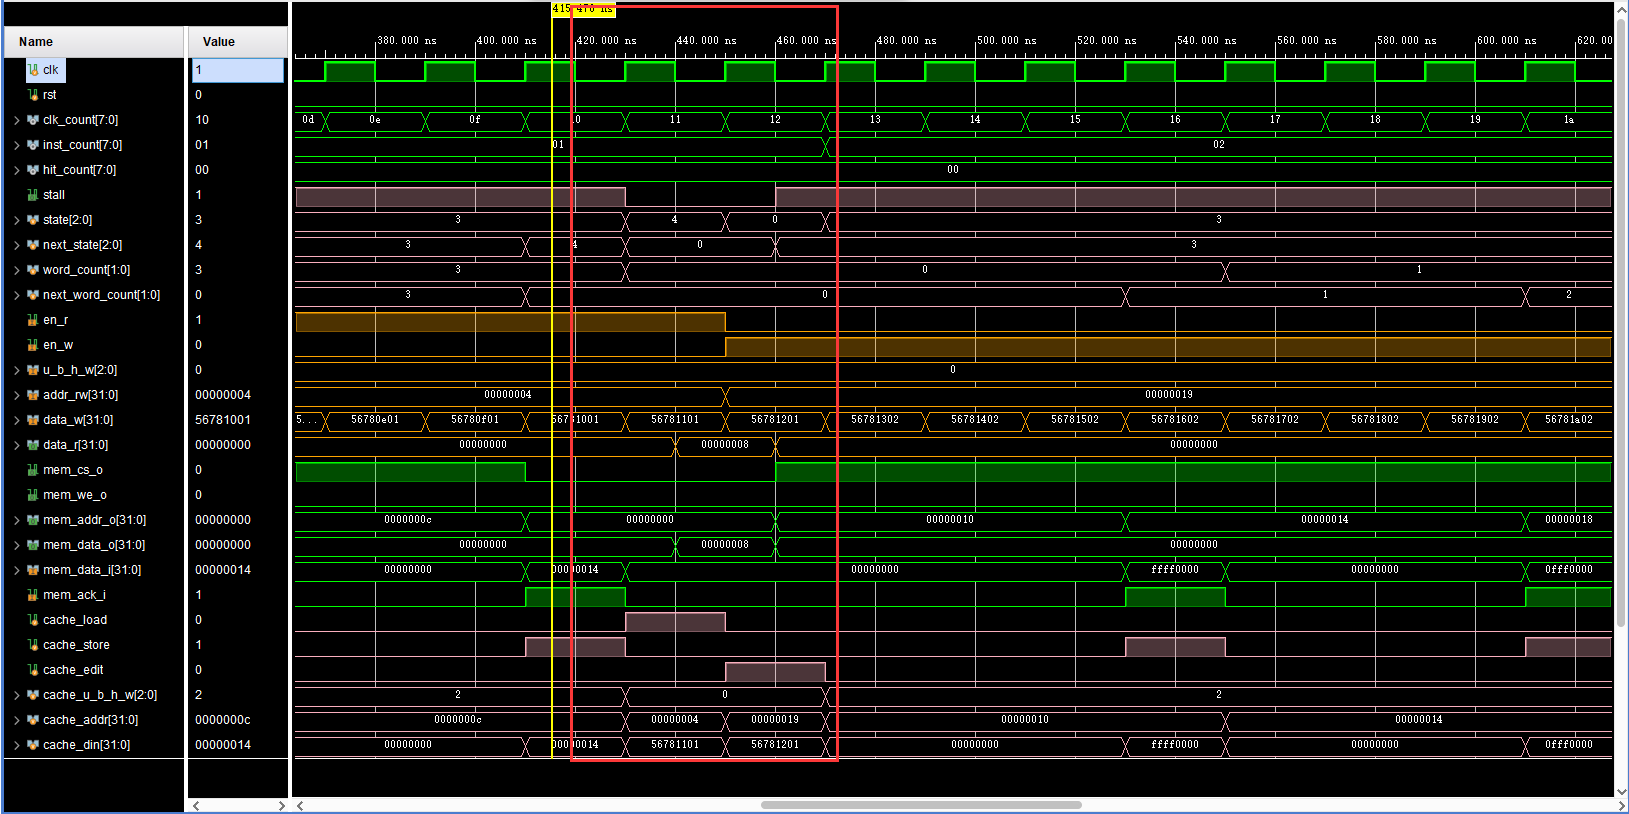
\includegraphics[width=1.0\textwidth]{figs/sres5.png}
    \caption{write miss}
    \label{Fig.8}
\end{figure}

之后的同样进入S\_FILL阶段,此阶段与前类似,在此不再赘述。此后进入S\_WAIT状态,此时cache\_edit信号升起,并且
cache\_addr也被修改为对应地址,仿真结果正确

\begin{figure}[H]
    \centering
    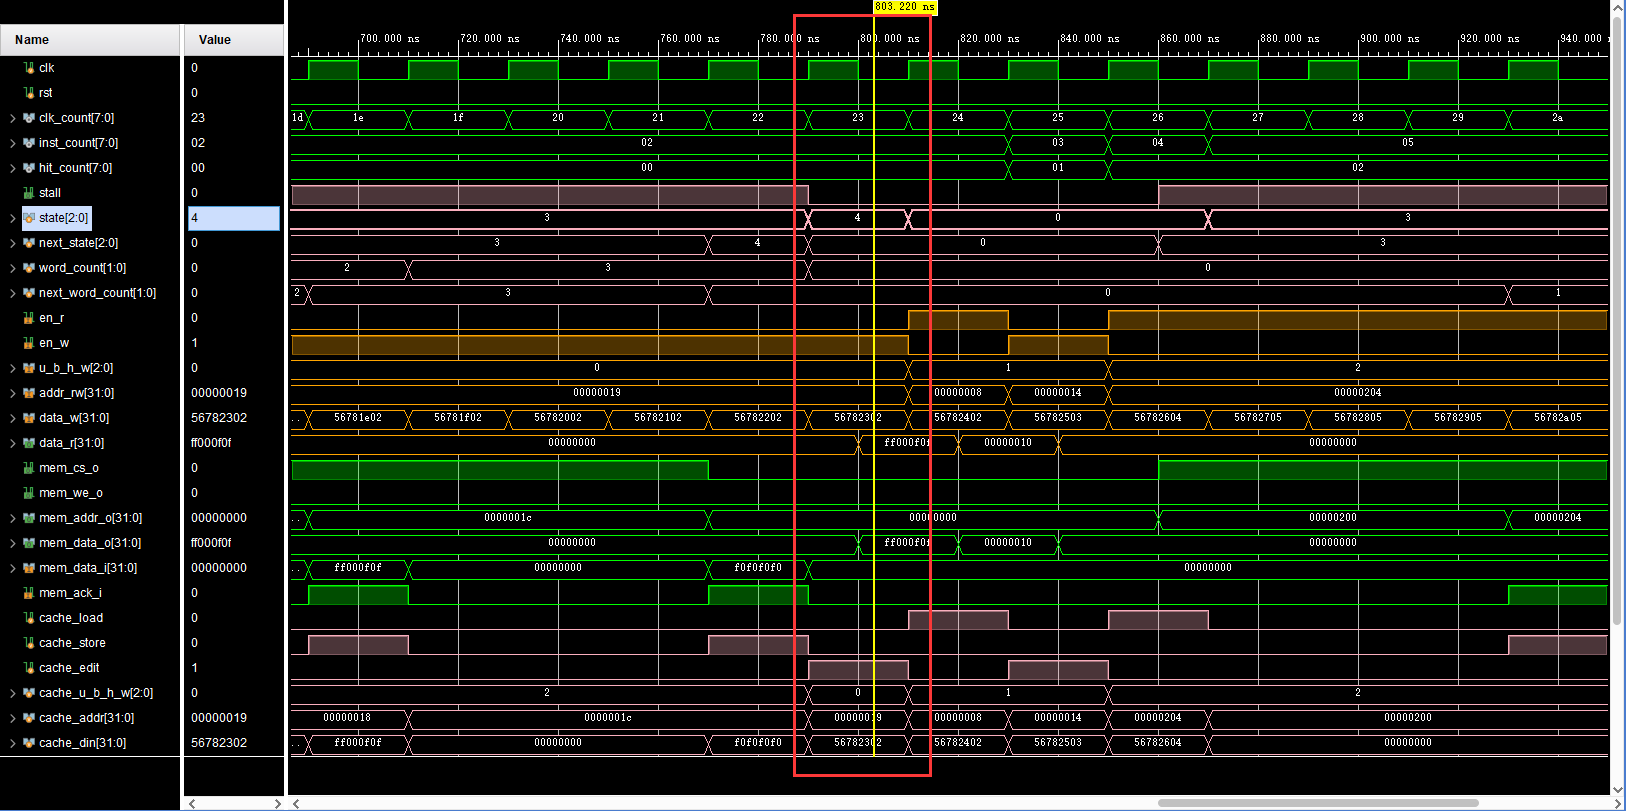
\includegraphics[width=1.0\textwidth]{figs/sres6.png}
    \caption{S\_WAIT}
    \label{Fig.9}
\end{figure}

read hit与write hit的情形仅需一个时钟周期就可以完成,对应的使能信号升起,
cache的addr和din/dout也被修改为对应值,从图中可以看到仿真结果正确。

\begin{figure}[H]
    \centering
    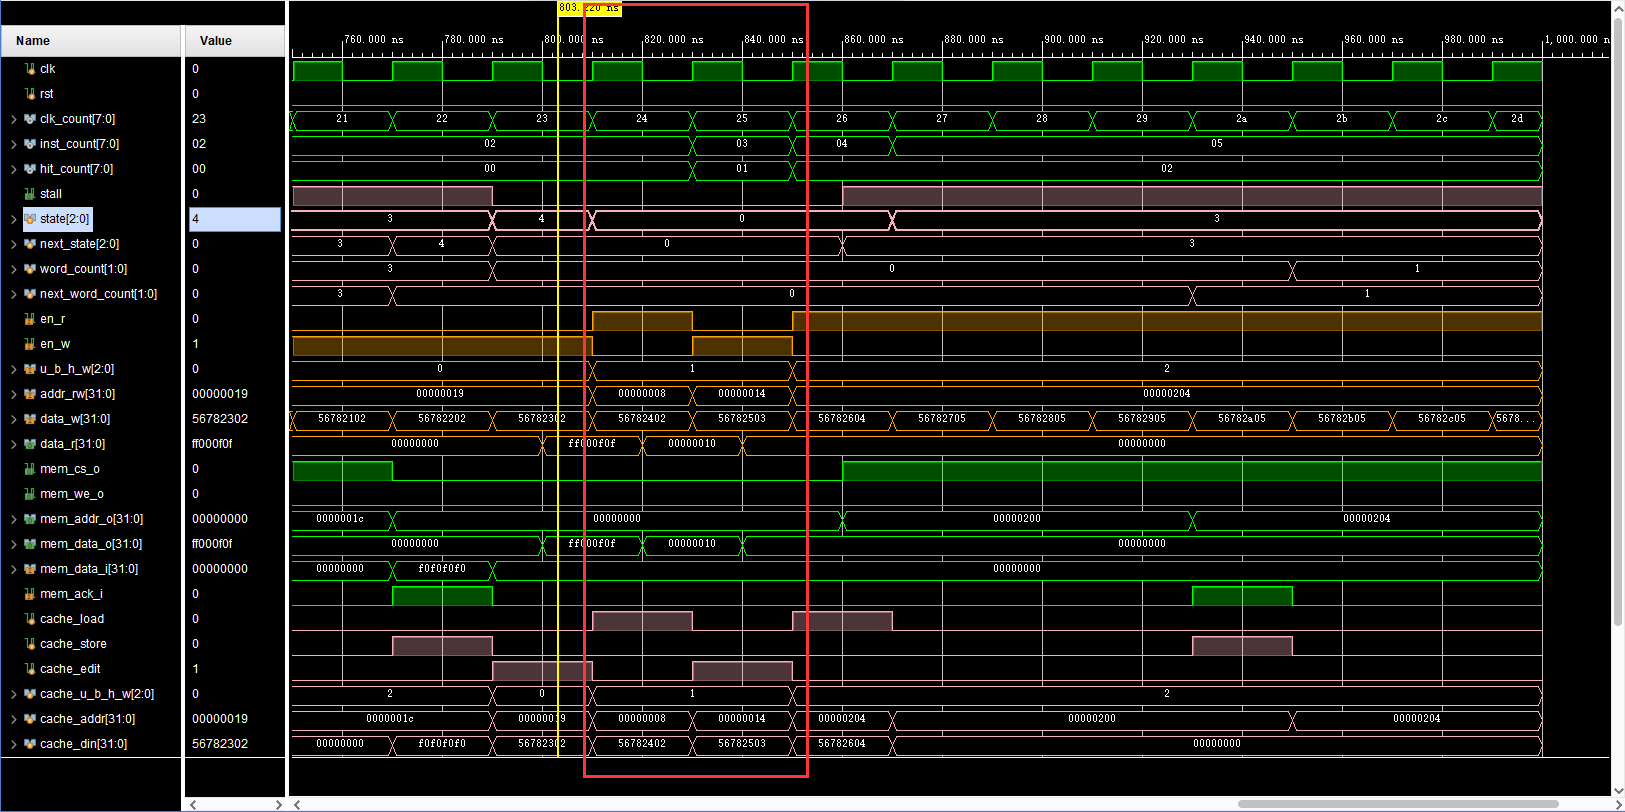
\includegraphics[width=1.0\textwidth]{figs/sres7.png}
    \caption{read hit}
    \label{Fig.10}
\end{figure}

下面再来检查dirty情形cache的正确性,经过一系列操作之后再读取脏块,
可以看到state下一周期被置为了2(S\_BACK),S\_BACK在上升沿将上个状态的数据写回到memory,
下降沿从cache读下次需要写回的数据(因此最后一次读无意义),
由计数器控制直到整个cache line全部写回。由于memory设置为4个周期完成读写操作,因此需要等待memory给出ack信号,才能进行状态的改变。
由于一个Data line有4个Word而一个Word同样需要4个周期写回,所以此过程需要额外经历一个S\_PRE\_BACK状态和16个时钟周期的S\_BACK状态,
然后再类似与上述情形经历16周期S\_FILL状态和S\_WAIT状态,仿真结果正确。

\begin{figure}[H]
    \centering
    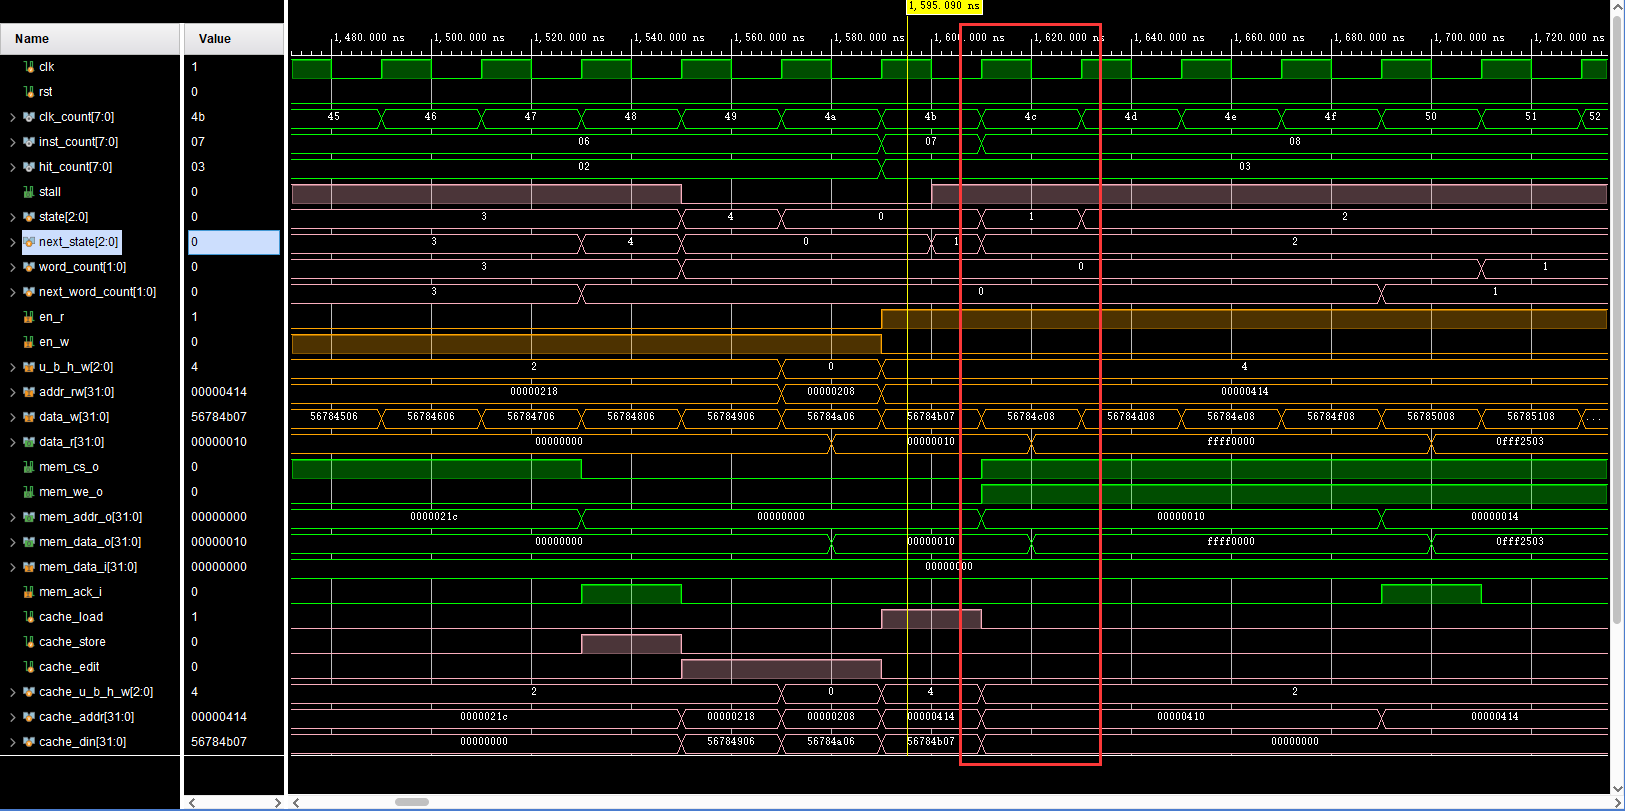
\includegraphics[width=1.0\textwidth]{figs/sres8.png}
    \caption{S\_PRE\_BACK}
    \label{Fig.11}
\end{figure}

\begin{figure}[H]
    \centering
    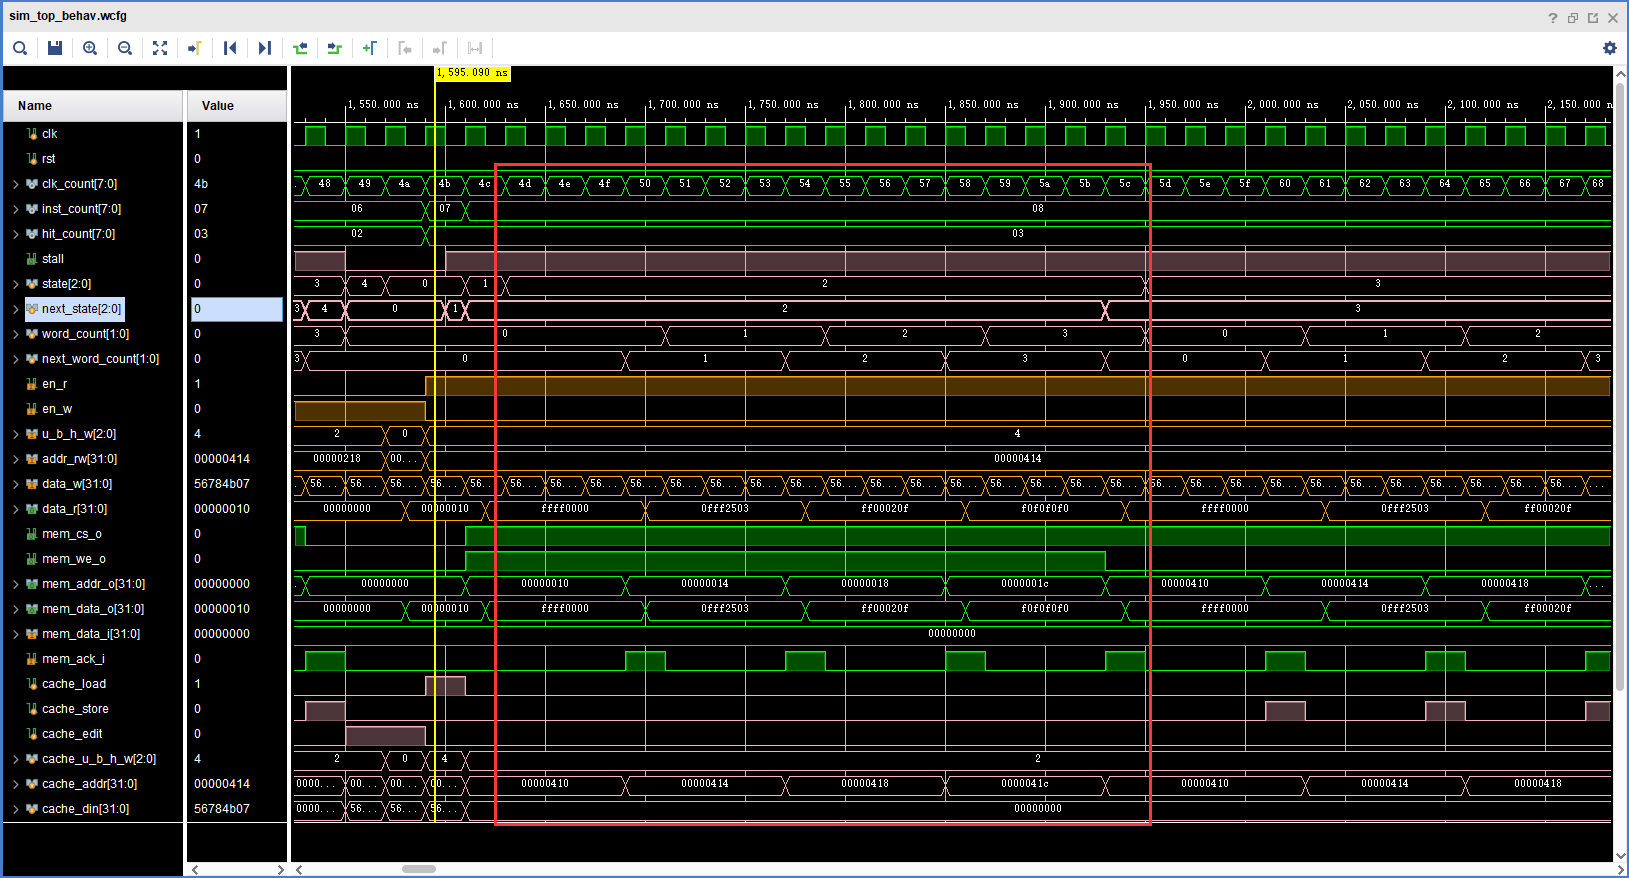
\includegraphics[width=1.0\textwidth]{figs/sres9.png}
    \caption{S\_BACK}
    \label{Fig.12}
\end{figure}

\begin{figure}[H]
    \centering
    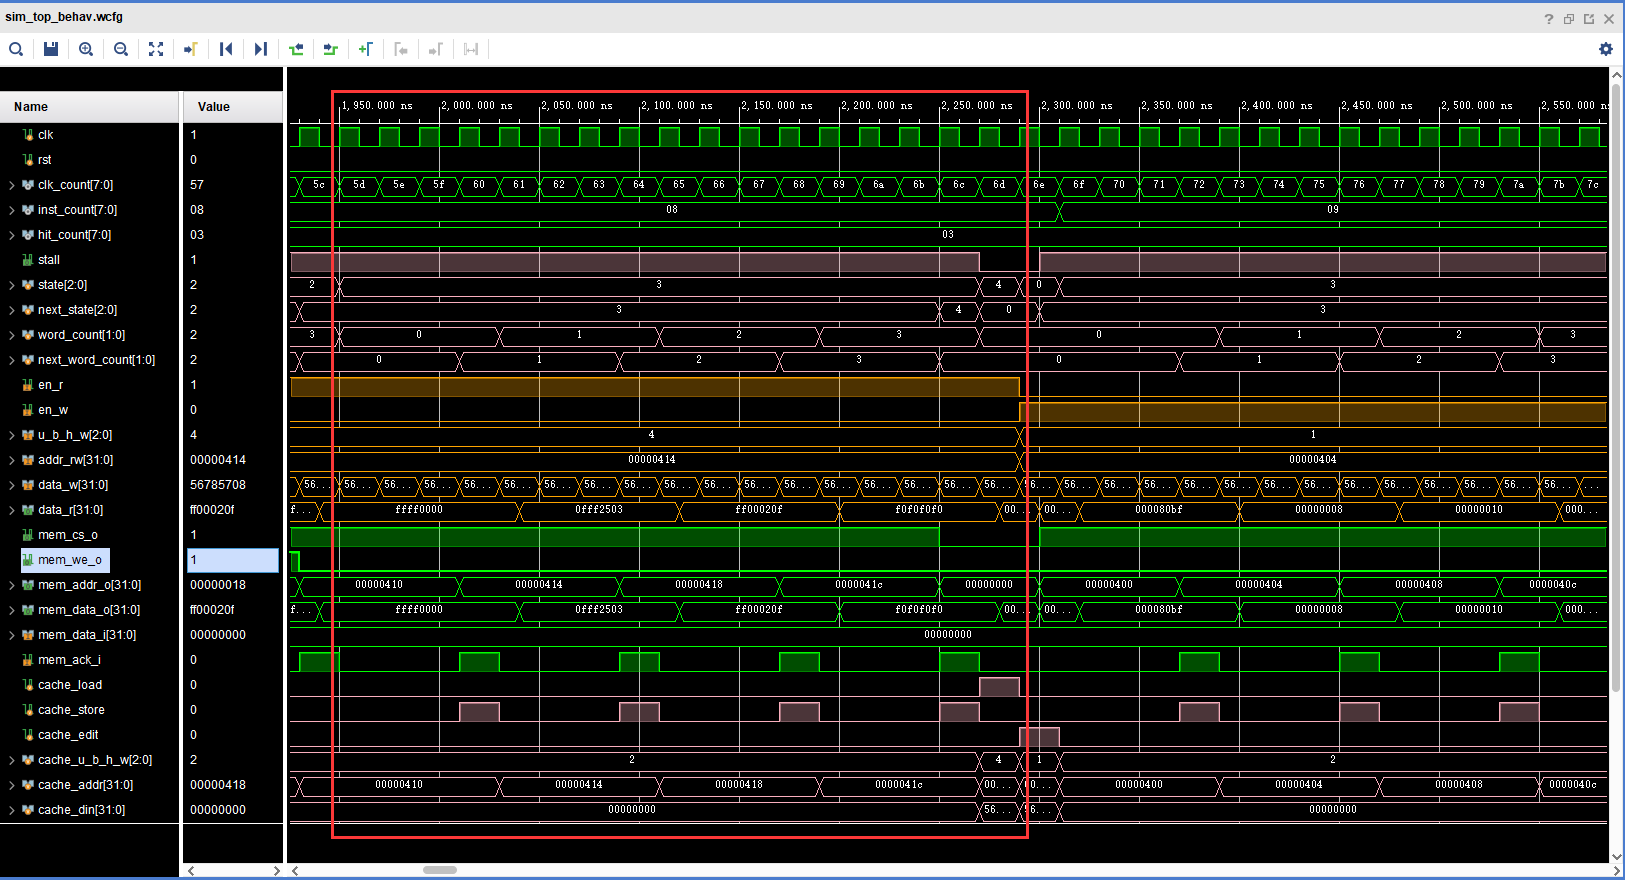
\includegraphics[width=1.0\textwidth]{figs/sres10.png}
    \caption{S\_FILL and S\_WAIT}
    \label{Fig.13}
\end{figure}

\subsection{上板结果分析}
仿真结果正确已经基本验证了实验的正确性,下面我组再简单的通过几张结果截图分析正确性。

指令流进MEM阶段之前不做处理
\begin{figure} [H]
    \centering
    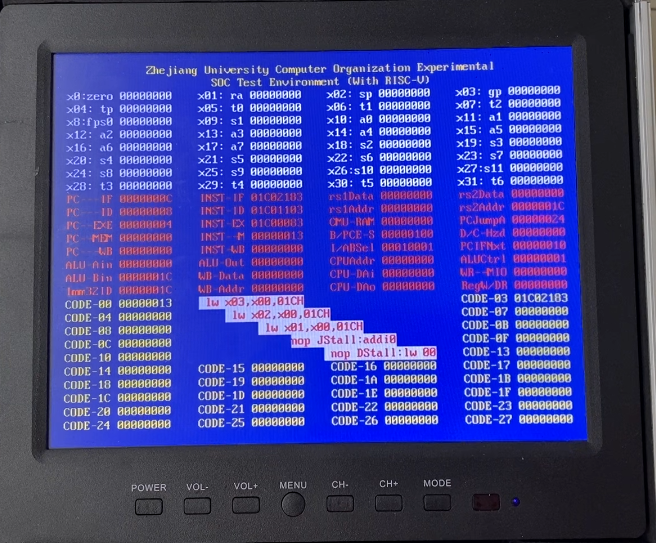
\includegraphics[width=1.0\textwidth]{figs/res1.png}
    \caption{res1}
    \label{Fig.14}
\end{figure}

第一条load指令进入MEM阶段后会花16个周期进行S\_FILL阶段,从CMU\_RAM的值可以看到
每次读一个Word都是从00030001增加到00030003,其中第四位是state,最后一位是word\_count

\begin{figure}[H]
    \centering
    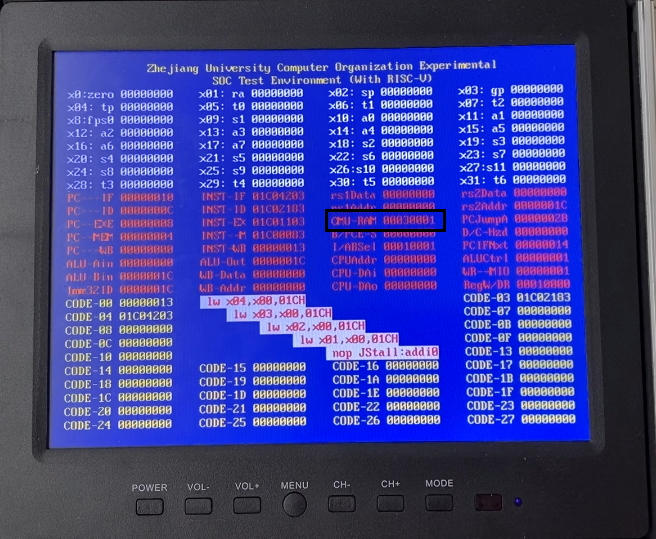
\includegraphics[width=1.0\textwidth]{figs/res2.png}
    \caption{res2}
    \label{Fig.15}
\end{figure}

S\_FILL之后会进入到S\_WAIT状态,如下图所示:
\begin{figure}[H]
    \centering
    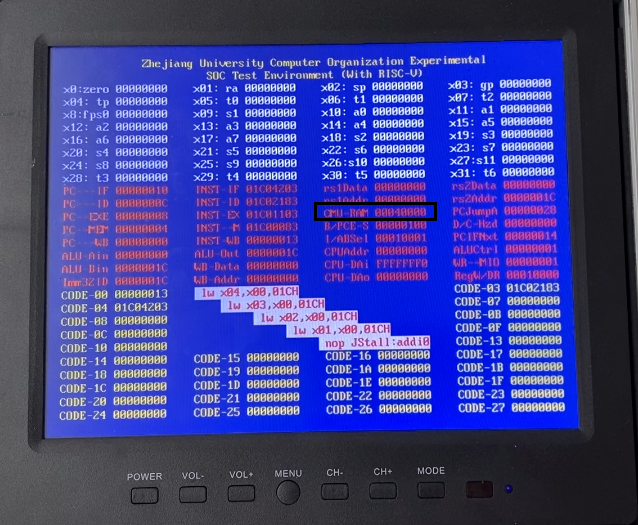
\includegraphics[width=1.0\textwidth]{figs/res3.png}
    \caption{res3}
    \label{Fig.16}
\end{figure}

当脏块需要写回时,会进入S\_PRE\_BACK状态,如下图所示:
\begin{figure}[H]
    \centering
    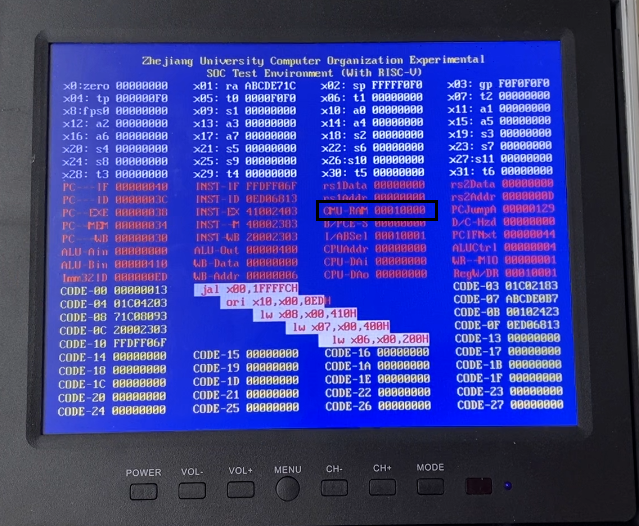
\includegraphics[width=1.0\textwidth]{figs/res4.png}
    \caption{res4}
    \label{Fig.17}
\end{figure}

之后会进入S\_BACK状态,如下图所示:
\begin{figure}[H]
    \centering
    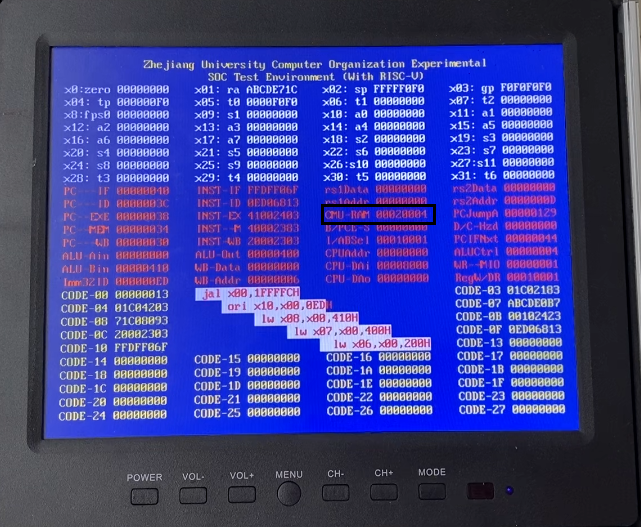
\includegraphics[width=1.0\textwidth]{figs/res5.png}
    \caption{res5}
    \label{Fig.18}
\end{figure}

后续的流程类似,均符合上部分仿真结果,具体流程会在验收时展示。